%\documentclass[11pt,fleqn]{book}%
%\documentclass{exam}%
\documentclass[11pt,a4paper]{article}
\date{{\LARGE Aprile 2019}}
\usepackage[italian]{babel}
\usepackage[T1]{fontenc}
\usepackage{graphicx}
\usepackage[11pt]{moresize}

\font\myfont=cmr12 at 40pt
\title{{\myfont Sezione d'urto}}

\author{{\Huge Francesco Sacco}\\ \\ \\
		
\includegraphics[scale=0.6]{Immagini/cherubino.eps}\\}
\usepackage[utf8x]{inputenc}
\usepackage{amsmath}
\usepackage{amsthm}
\usepackage{hyperref}

\newcommand{\vettore}[1]{\mathbf{#1}}
\newcommand{\vettorec}[1]{\textrm{#1}}
\newcommand{\pscal}[2]{\langle \vettore{#1},\vettore{#2}\rangle}

\begin{document}
	\maketitle
	\newpage
	\section*{Prefazione}
		Visto che c'è molta confusione sulla sezione d'urto faccio questi brevi appunti per chiarire bene cos'è e cosa rappresenta.\newline
		Lungo il pdf mettero un bel pò di note a piè di pagina, esse vanno lette solo se non si capisce quello che si sta leggendo, se stai capendo non leggerle,\footnote{Minchia ma allora non hai capito un cazzo} rovinano il flusso della discussione.\newline 
		La sezione d'urto viene indicata di solito con $\sigma$, Il suo nome richiama alla mente qualcosa che abbia a che vedere un'area su cui sbatte qualcosa. Però la sezione d'urto non è sempre l'area dell'oggetto, ma intende rappresentare una sorta di "area equivalente".\newline
		Ad esempio è ragionevole dire che per la luce l'area effettiva di un vetro $1m\times 1m$ è minore di un metro quadro, questo perchè molti fotoni passano attraverso il vetro indisturbati.\newline
	\section{Sezione d'urto s'un oggetto opaco}
	\label{sec:opaco}
		Per semplicità iniziano a trattare il concetto di sezione d'urto nel caso di un oggetto opaco,\footnote{Chiaramente le particelle incidenti sono fotoni, ma con un pò di fantasia si può generalizzare il concetto con oggetti incidenti diversi dai fotoni} in questo caso ci aspettiamo che la sezione d'urto sia uguale alla superfice ortogonale al facio.\newline
		Noi in questo caso vogliamo ricavare l'area ortogonale in base a quello che succede al fascio di luce che lo colpisce.\newline

		Supponiamo di mandare un facio di luce con un'area maggiore del bersaglio, e che dietro ci sia uno schermo ortogonale al facio molto grande che raccolga la luce (figura \ref{fig:ombra}), allora possiamo dire che la sezione d'urto è l'area dell'ombra che l'oggetto genera sullo schermo.\newline
		Chiamarente se l'oggetto è una superfice orientata ortogonalmente al facio luminoso, la sua sezione d'urto sarà uguale alla sua area.\newline
		\begin{figure}
			\centering
    		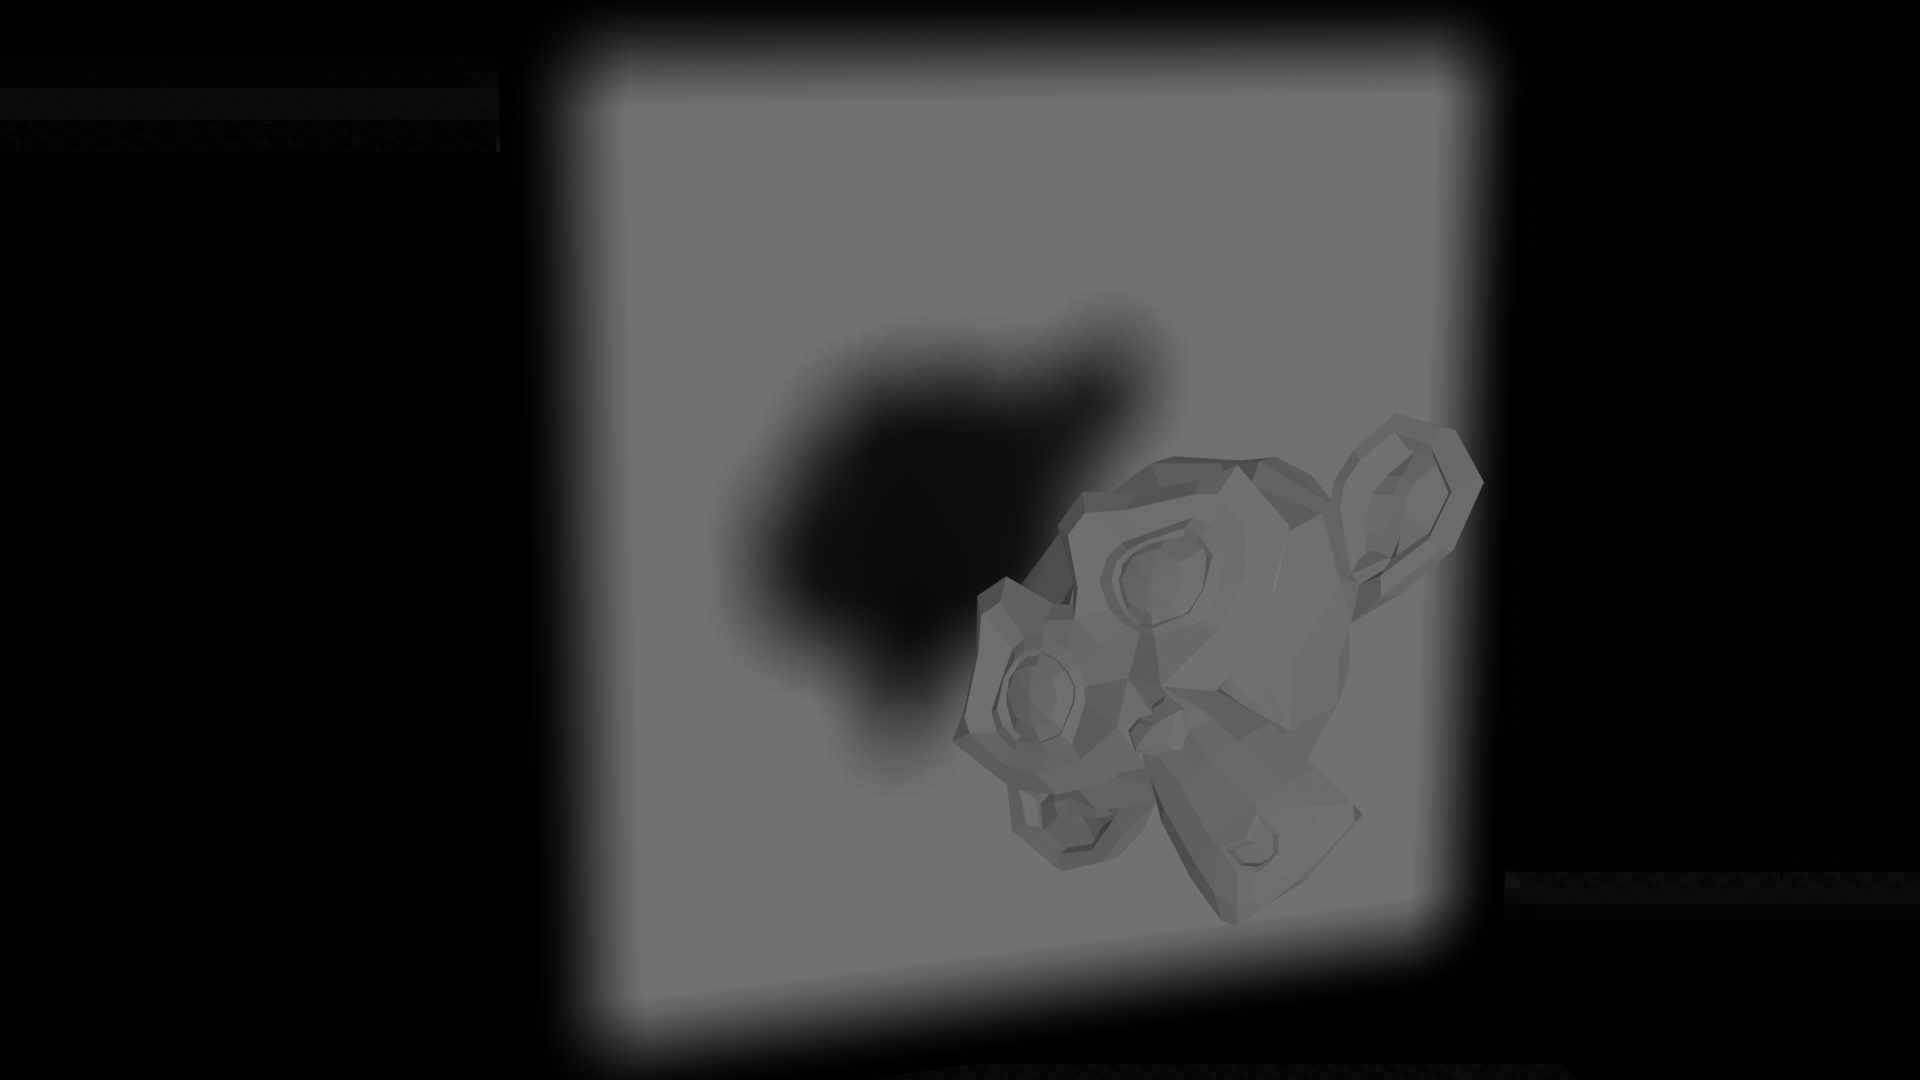
\includegraphics[width=\linewidth]{Immagini/ombra_con_blender.png}
    		\caption{Immagine fatta male illustrativa}
    		\label{fig:ombra}
		\end{figure}

		Solo che c'è un problema: nel caso di un'oggetto sgummato sarà difficile misurare l'area. Per ovviare a questo problema si può mettere uno schermo che sia in grado di contare i fotoni che riceve e una sorgente che sia in grado di contare i fotoni che manda.\newline
		Chiamiamo $A$ l'area illuminata dalla sorgente quando non c'è il bersaglio in mezzo ai piedi, che per comodità la creiamo quadrangolare, $n_s$ il numero di fotoni che colpiscono lo schermo per unità di tempo e $\Phi$ il numero di fotoni che vengono sparati dalla luce per unità di tempo, allora con una semplice proporzione si può dire che:
		\begin{equation}
			\sigma:(n_l-n_s)=A:n_l \rightarrow \sigma=A\times(1-n_s/\Phi)
			\label{eq:sigma_luce}
		\end{equation}
		Adesso vediamo se funziona veramente questo ragionamento.\newline
		Per verificare prendiamo un bersaglio quadrato di area $\sigma=1$ illuminata da una luce quadrata di area $A=2$, di conseguenza metà dei fotoni verrà bloccata, cioè $n_s=\Phi/2$, quindi $1=2\times(1-\Phi/2\times 1/\Phi)=2\times(1-1/2)=2\times 1/2=1$.\newline
		Che bello funziona.\newline

		Una cosa molto importante che poi verrà applicata è l'additività della sezione d'urto, infatti se prendiamo due schermi opachi quadrati con $\sigma=1$ e li mettiamo uno accanto all'altro formando un rettangolo, esso avrà una sezione d'urto uguale a $2$.

	\section{Sezione d'urto s'un oggetto traslucido}
		Per gli oggetti traslucidi tratteremo soltanto quelli planari, perchè quelli con geometri tridimenzionali si comportano in modo strano con la luce.\footnote{Facendo qualche assunzione volendo si potrebbe trattare anche oggetti tridimenzionali, ma non credo aiuti alla comprenzione del testo}\newline

		Se ti dico:"Io ho una lastra di vetro di un metro quadro che fa passare la metà della luce, qual'è la sezione d'urto?"\footnote{Supponiamo che la luce che non passi venga assorbita, a dire il vero non è molto importante che fine faccia} tu mi risponderai di sicuro:"mezzo metro quadro", ma come è possibile giustificare questa affermazione?\newline

		Chiaramente deriva dall'equazione \ref{eq:sigma_luce}, ma si perde un pò il concetto che invece era ben chiaro con lo schermo opaco che ci ha portato in primo luogo a ricavare quell'equazione.\newline

		Ora però ti porto un'altro vetro traslucido con le esatte stesse proprietà, e ti chiedo:"qual'è la sezione d'urto di quest'altro vetro?", tu mi dirai:"è lo stesso di prima, quindi per forza sarà mezzo metro quadro", e io ti rispondo:"la tua sezione d'urto è esatta, ma ti sbagli a dire che è lo stesso di prima! Questo è uno schermo opaco che ha tantissimi buchetti microscopici che in totale gli levano metà dell'area"\footnote{Chiaramente è un'esperimento mentale, nella realtà fare una cosa del genere non sarà possibile perchè dovrebbe avere uno spessore nullo e la luce ha anche un comportamento ondulatorio che porterebbe alla diffrazione, ma possiamo supporre che tutto questo non accada in questo esempio}.\newline

		Quindi effettivamente possiamo dire che il vetro è un pò come uno schermo opaco con tanti buchettini, e quindi deve avere la stessa sezione d'urto, e quindi si usa l'equazione \ref{eq:sigma_luce}.\newline

	\section{Collegamento con la probabilità}
		Sempre rimandendo nel caso del vetro traslucido posso fare questa affermazione:Se il fotone viene assorbito, allora vuol dire che ha interagito con un'atomo dell vetro, altrimenti è passato indisturbato.\newline

		Ora vogliamo vedere se è possible legare la probalbilirà di interazione $P$ con la sezione d'urto.\newline
		Sempre usando la notazione della sezione \ref{sec:opaco} e dell'equazione \ref{eq:sigma_luce}, possiamo dire che la probabilità $P$ che il fotone incida sia quanti ne vengono assorbiti dal bersaglio per unità di tempo, che sono tanti quanti a quellli che non arrivano sullo schermo per unità di tempo $N_i=(\Phi-n_s)$, diviso quanto ne arrivano in totale $\Phi$, quindi:
		\begin{equation}
			P=\frac {N_i} \Phi=\Big(1-\frac {n_s}\Phi\Big)=\frac\sigma A
			\label{eq:prob1}
		\end{equation}

	\section{Sezione d'urto di una particella}
		Supponiamo adesso che la luce venga proiettata in modo che ogni singolo fotone colpisca il bersaglio (ma non per forza deve essere assorbito, può anche attraversarlo se è translucito), e che il bersaglio sia un oggetto planare con una densità di atomi per unità di superfice $n_s$.\newline
		Adesso io voglio sapere quantè la sezione d'urto di un atomo sulla superfice, visto che la sezione d'urto è additiva\footnote{come spiegato negli ultimi righi del paragrafo \ref{sec:opaco}} posso dire che la sezione d'urto del bersagio $\sigma_b$ è uguale alla sezione d'urto di un singolo atomo $\sigma$ moltiplicato per quanti ce ne sono per unità di superfice $n_s$ moltiplicato per quanta superfice c'è $A$, quindi:
		\[
			\frac{AN_i}\Phi=\sigma_b=\sigma A n_s
		\]
		dove la prima eguaglianza viene dall'equazione \ref{eq:prob1}, risolvendo per sigma si ottiene che 
		\begin{equation}
			\sigma=\frac{N_i}{\Phi n_s}
		\end{equation}
		Questa equazione però dipende da come è fatta la lastra bersaglio, quindi se vogliamo qualcosa che ne sia indipendente bisogna fare qualche passaggio matematico:
		\[
			\sigma=\frac{N_i}{\Phi n_s}\times \frac{An_s}{An_s}=
			\frac{N_i}{An_s}\times\frac A\Phi\times \frac {n_s}{n_s}=
			N_a\times \frac1{|j|}\times 1=\frac{N_a}{|j|}
		\]
		Dove ho detto che il numero di interazioni sulla lastra per unità di tempo $N_i$ è uguale al numero di interazioni su un singolo atomo $N_a$ moltiplicato per quanti atomi ci sono $An_s$ (Area per densità), quindi $N_i/(An_s)=N_a$ e poi ho detto che il flusso attraverso l'area $\Phi$ diviso l'area stessa $A$ dà la densità di corrente, quindi $A/\Phi=1/|j|$.\newline
		Mettendo tutti insieme si ha che 
		\begin{equation}
			\sigma=\frac{N_a}{|j|}
		\end{equation}


		

\end{document}